\subsection{BenchCouncil BigDataBench}
{{\footnotesize
\noindent BigDataBench provides benchmarks for evaluating big data and AI workloads with realistic datasets (13 sources) and pipelines across analytics, graph, warehouse, NoSQL, streaming, and AI.


\begin{description}[labelwidth=4cm, labelsep=1em, leftmargin=4cm, itemsep=0.1em, parsep=0em]
  \item[date:] 2020-01-01
  \item[version:] v1.0
  \item[last\_updated:] 2020-01
  \item[expired:] unknown
  \item[valid:] yes
  \item[valid\_date:] 2020-01-01
  \item[url:] \href{https://www.benchcouncil.org/BigDataBench/}{https://www.benchcouncil.org/BigDataBench/}
  \item[doi:] 10.48550/arXiv.1802.08254
  \item[domain:] General
  \item[focus:] Big data and AI benchmarking across structured, semi-structured, and unstructured data workloads
  \item[keywords:]
    - big data
    - AI benchmarking
    - data analytics
  \item[licensing:] Apache License 2.0
  \item[task\_types:]
    - Data preprocessing
    - Inference
    - End-to-end data pipelines
  \item[ai\_capability\_measured:]
    - Data processing and AI model inference performance at scale
  \item[metrics:]
    - Data throughput
    - Latency
    - Accuracy
  \item[models:]
    - CNN
    - LSTM
    - SVM
    - XGBoost
  \item[ml\_motif:]
    - General
  \item[type:] Benchmark
  \item[ml\_task:]
    - NA
  \item[solutions:] Solution details are described in the referenced paper or repository.
  \item[notes:] Built on eight data motifs; provides Hadoop, Spark, Flink, MPI implementations.

  \item[contact.name:] Jianfeng Zhan (BenchCouncil)
  \item[contact.email:] unknown
  \item[results.links.name:] ChatGPT LLM
  \item[results.links.url:] \href{https://docs.google.com/document/d/1VFRxhR2G5A83S8PqKBrP99LLVgcCGvX2WW4vTtwxmQ4/edit?usp=sharing}{https://docs.google.com/document/d/1VFRxhR2G5A83S8PqKBrP99LLVgcCGvX2WW4vTtwxmQ4/edit?usp=sharing}
  \item[fair.reproducible:] Yes
  \item[fair.benchmark\_ready:] Yes
  \item[id:] benchcouncil\_bigdatabench
  \item[Citations:] \cite{gao2018bigdatabenchscalableunifiedbig}
\end{description}

{\bf Ratings:} ~ \\

\begin{tabular}{p{0.15\textwidth} p{0.07\textwidth} p{0.7\textwidth}}
\hline
Rating & Value & Reason \\
\hline
dataset & 4 & Some datasets lack consistent versioning or rich metadata annotations.
 \\
documentation & 4 & Setup requires manual steps; some task-specific instructions lack clarity.
 \\
metrics & 5 & None
 \\
reference\_solution & 4 & Not all benchmark components have fully reproducible baselines; deployment across platforms is fragmented.
 \\
software & 3 & No automated setup across all tasks; some components require manual integration.
 \\
specification & 4 & Specific I/O formats and hardware constraints are not uniformly detailed across all tasks.
 \\
\hline
\end{tabular}

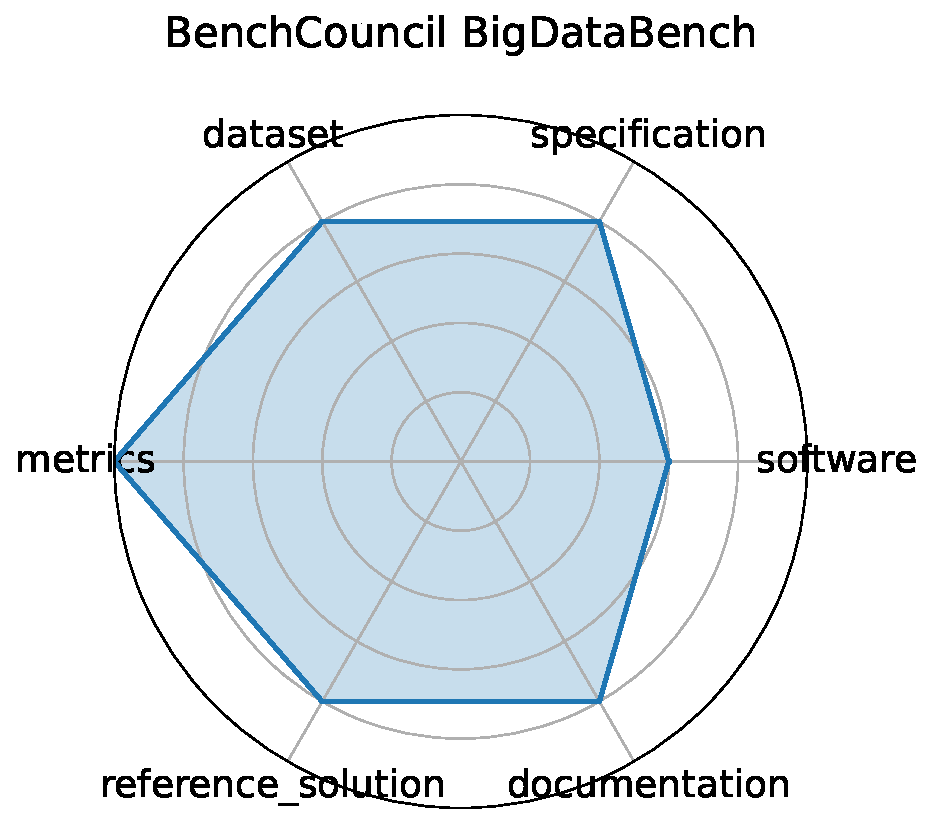
\includegraphics[width=0.2\textwidth]{benchcouncil_bigdatabench_radar.pdf}
}}
\clearpage